
%(BEGIN_QUESTION)
% Copyright 2013, Tony R. Kuphaldt, released under the Creative Commons Attribution License (v 1.0)
% This means you may do almost anything with this work of mine, so long as you give me proper credit

Plott responsen for følgende PD-regulator (Proporsjonal + Derivat) på en trinnvis endring i prosessvariabelen. Anta revers virkemåte, gain = 2 ($PB = 50\%$), derivat $\tau_d = 1.0$ minutt, og bias = 30\%:

$$\includegraphics{i01815x01.eps}$$

\underbar{file i01815}
%(END_QUESTION)





%(BEGIN_ANSWER)

$$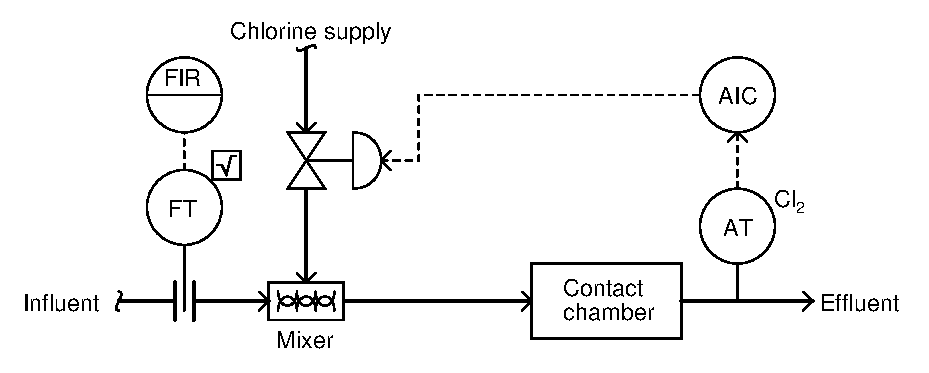
\includegraphics[width=10cm]{i01815x02.eps}$$

%(END_ANSWER)





%(BEGIN_NOTES)

Det kan være lurt å be studentene tegne P-responsen og D-responsen hver for seg, og deretter summere dem algebraisk for å få den endelige utgangsresponsen.

%INDEX% Control, proportional + derivative: graphing controller response

%(END_NOTES)
